\documentclass[class=article,11pt,border=6pt]{standalone}
% Standalone build of Figure 2 of "The Router Already Knows".
% The picture code is copied verbatim from the paper's source.
\usepackage[T1]{fontenc}
\usepackage[sc]{mathpazo}
\linespread{1.045}
\usepackage{amsmath,amssymb}
\usepackage{xcolor}
\usepackage{tikz}
\usetikzlibrary{arrows.meta,calc}
\usepackage{pgfplots}
\pgfplotsset{compat=1.17}
\usepgfplotslibrary{groupplots}
\begin{document}
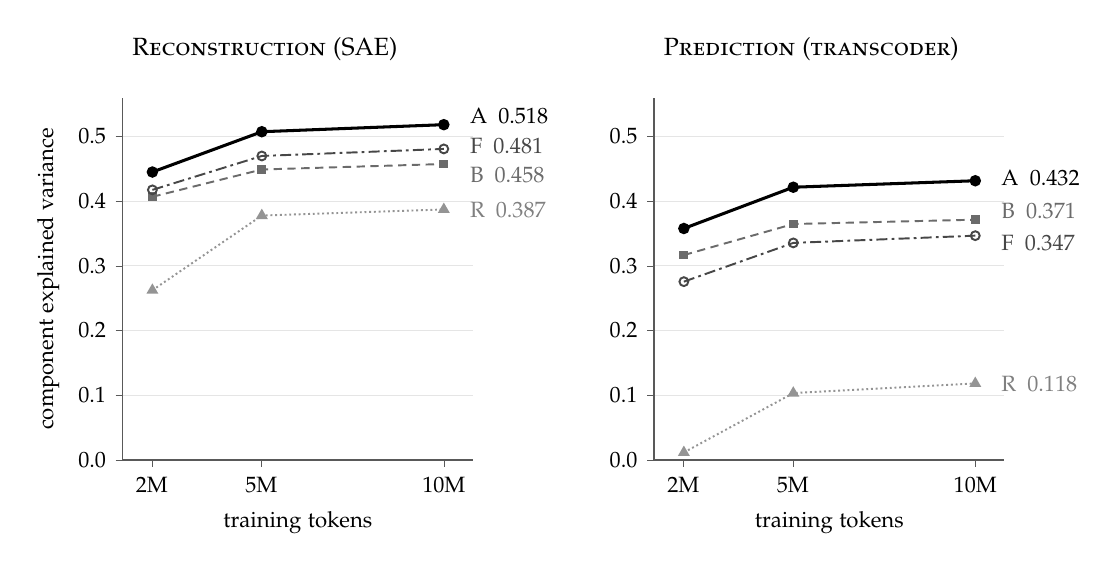
\begin{tikzpicture}
\pgfplotsset{
  styA/.style={black, line width=1.1pt, mark=*, mark size=1.5pt},
  styF/.style={black!72, line width=0.7pt, dash pattern=on 4pt off 1.5pt on 1pt off 1.5pt,
               mark=o, mark size=1.6pt, mark options={solid, fill=white}},
  styB/.style={black!58, line width=0.7pt, dash pattern=on 3pt off 2pt,
               mark=square*, mark size=1.25pt, mark options={solid}},
  styR/.style={black!42, line width=0.7pt, densely dotted,
               mark=triangle*, mark size=1.8pt, mark options={solid}},
}
\tikzset{
  endlabA/.style={anchor=west, font=\footnotesize, text=black},
  endlabF/.style={anchor=west, font=\footnotesize, text=black!72},
  endlabB/.style={anchor=west, font=\footnotesize, text=black!58},
  endlabR/.style={anchor=west, font=\footnotesize, text=black!50},
}
\begin{groupplot}[
  group style={group size=2 by 1, horizontal sep=23mm},
  scale only axis, width=4.45cm, height=4.6cm,
  xmin=1.2, xmax=10.8, ymin=0, ymax=0.56,
  xtick={2,5,10}, xticklabels={2M,5M,10M},
  ytick={0,0.1,0.2,0.3,0.4,0.5},
  yticklabel style={/pgf/number format/fixed,/pgf/number format/fixed zerofill,/pgf/number format/precision=1},
  axis lines=left, axis line style={black!65, line width=0.45pt, -},
  tick style={black!65}, tick align=outside, major tick length=2.5pt,
  ymajorgrids, major grid style={black!10, line width=0.35pt},
  every tick label/.append style={font=\footnotesize},
  label style={font=\footnotesize},
  xlabel={training tokens},
  title style={font=\small\scshape, anchor=south west, at={(0,1.03)}},
  clip=false,
]
\nextgroupplot[title={Reconstruction (SAE)}, ylabel={component explained variance}]
\addplot[styR] coordinates {(2.0152,0.2624) (5.0135,0.3779) (10.0000,0.3873)};
\addplot[styB] coordinates {(2.0152,0.4069) (5.0135,0.4491) (10.0000,0.4576)};
\addplot[styF] coordinates {(2.0152,0.4176) (5.0135,0.4700) (10.0000,0.4809)};
\addplot[styA] coordinates {(2.0152,0.4452) (5.0135,0.5075) (10.0000,0.5184)};
\node[endlabA] at (axis cs:10.45,0.532) {A\enspace0.518};
\node[endlabF] at (axis cs:10.45,0.486) {F\enspace0.481};
\node[endlabB] at (axis cs:10.45,0.440) {B\enspace0.458};
\node[endlabR] at (axis cs:10.45,0.387) {R\enspace0.387};
\nextgroupplot[title={Prediction (transcoder)}]
\addplot[styR] coordinates {(2.0152,0.0116) (5.0135,0.1034) (10.0000,0.1183)};
\addplot[styB] coordinates {(2.0152,0.3168) (5.0135,0.3648) (10.0000,0.3715)};
\addplot[styF] coordinates {(2.0152,0.2757) (5.0135,0.3356) (10.0000,0.3468)};
\addplot[styA] coordinates {(2.0152,0.3579) (5.0135,0.4217) (10.0000,0.4317)};
\node[endlabA] at (axis cs:10.45,0.436) {A\enspace0.432};
\node[endlabF] at (axis cs:10.45,0.336) {F\enspace0.347};
\node[endlabB] at (axis cs:10.45,0.385) {B\enspace0.371};
\node[endlabR] at (axis cs:10.45,0.118) {R\enspace0.118};
\end{groupplot}
\end{tikzpicture}
\end{document}
